\section{Simple, Continuous Domains}
\subsection{Overview of the problem}
The Pole Balancing problem, sometimes referred to as the inverted pendulum, is another canonical problem of reinforcement learning.  The paper “The Pole Balancing Problem, A Benchmark Control Theory Problem” (Brownlee, 2005) contains a detailed description of the standard definition of the problem that was used in this project.  In the Pole Balancing problem, the state consists of a cart on a track with a vertical pole attached to a hinge on the cart.  The goal is to keep the pole balanced within a certain tolerance of the vertical position and to prevent the car from going off either end of the track by applying a fixed force to either end of the car (see Figure~\ref{fig:pole_diag}).  The state of the world consists of four continuous values: the position and velocity of the cart and the angle and angular velocity of the pole.  The agent has no knowledge of how the world works and chooses between two actions: apply the fixed force to the left or to the right.

\end{flushleft}

\begin{figure}[hbtp]
\center
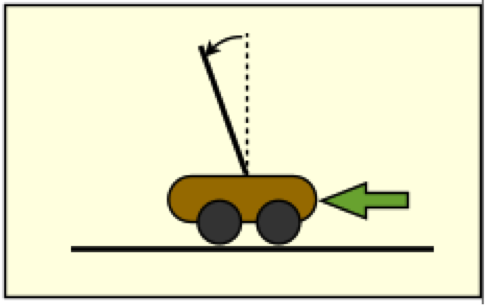
\includegraphics[scale=0.5]{fig06}
\caption{Pole balancing problem}
\label{fig:pole_diag}
\end{figure}

\begin{flushleft}

A reward is introduced to make this a reinforcement learning problem.  The reward is 0 for every time step that the car is on the track and the pole is in the allowable vertical range.  The agent receives a large negative reward if there is a failure due to the car running off the track, or the pole falling beyond the vertical tolerance.  Each trial begins with the state variables being initialized with random values.

This problem poses a new challenge due to the continuous state variables.  There are a number of ways that continuous variables can be handled.  One approach would be to learn a continuous function, $Q(s,a)$, over the continuous domain of the states.  This approach will be used in Chapter ??? .  For this problem we choose to partition the continuous states into a small number of cells.  The position and angle values are partitioned into 3 value ranges.  The cart velocity and angular velocity of the pole are partitioned into two value ranges, positive and negative.  This creates 36 possible discrete states of for the system.  Given the two possible actions, there are a total of 72 state-action values.  This manageable number of state-action values makes it reasonable to try to learn the $Q(s,a)$ function using TD$(\lambda)$ learning.  In this problem the agent attempts to learn the value of $Q(s,a)$ for each state-action pair using eligibility traces.  Eligibility traces should speed learning on this problem as reaching the failure state is intuitively attributable to many prior actions and not just one bad choice.

\subsection{GPU Implementation}
Temporal difference learning with eligibility traces is a complex algorithm to implement on a GPU.  Each agent must maintain a number of values for each state-action pair: the estimated $Q$-value, the eligibility trace, the weight for the $Q$-value that will be used during sharing, and the random bias amount (discussed in next section).   In addition there are random number seeds and stored values for previous state and action.

It is more difficult to monitor the learning process as well.  The agent’s quality cannot be determined by inspection.  It can only be determined by testing, so the learning process must be paused and the agent tested for a statistically significant number of time-steps.  For this problem learning quality is defined as the average time to failure over a trial of 8,192 time-steps.  Testing was done following each sharing phase. 

\subsection{Sharing}
Sharing among agents for this problem is done in a straightforward manner.  After a period of learning, the $Q$-values are averaged over all agents.  The average is done on a weighted basis.  Each agent maintains a weight for each state-action pair.  The weight for agent $i$ is $wgt_i(s,a)$ and it is initialized to a constant value.  During the learning process, the agent weights are updated as follows:

\begin{equation}
wgt_i(s,a) \gets wgt_i(s,a)+\alpha\epsilon_i(s,a)
\end{equation}

During sharing, an average value for all agents for $Q(s,a)$ is calculated based on the following equation:

\begin{equation}
Q_{total}(s,a)={ {\sum_iQ_i(s,a)wgt_i(s,a)} \over {\sum_iwgt_i(s,a)} }
\end{equation}

The value $Q_{total}(s,a)$ is shared with all agents and their weights are reset after sharing to the same constant initial value. 

\begin{equation}
Q_i(s,a) \gets Q_{total}(s,a)
\end{equation}

\begin{equation}
wgt_i(s,a) = \mbox{\it initial-wgt}
\end{equation}

\subsection{Differentiation}
The sharing described above produces identical agents at the start of each learning period.  Differentiation was added to the agents for this problem with beneficial results.  With differentiation, a small random bias amount is added to each agent’s $Q_i(s,a)$ values.  The amount of bias is added after sharing and it decreases over time.  The sharing update rules with differentiation are as follows, where $Rand(-1.0,1.0)$ is a uniform random number over the specified interval, {\it max-bias} is the maximum bias amount and {\it bias-decay-factor} controls the rate of reduction in the maximum bias:

\begin{equation}
Q_i(s,a) \gets Q_{total}(s,a) + Rand(-1.0,1.0) \times \mbox{\it max-bias}
\end{equation}

\begin{equation}
\mbox{\it max-bias} \gets \mbox{\it max-bias} / \mbox{\it bias-decay-factor}
\end{equation}

Randomly biasing the values of $Q(s,a)$ has the most impact on states where $Q(s,LEFT)$ is close to $Q(s,RIGHT)$, i.e. when the values learned so far do not clearly favor one action over the other.  In this situation, the random bias will cause some agents to choose $LEFT$ as the best action and others to choose $RIGHT$, generating new information about both actions from that state.  This, hopefully, leads to identifying one action as clearly the best when the agents pool their information at the next sharing point.  The next section shows the improvement in learning due to differentiation.

\subsection{Results}
Agent quality was measured for this problem as the average time to failure over 8,192 time steps.  Testing is required to determine agent quality as it cannot be determined by inspection.  Each agent is given a random starting state and runs for 8,192 time steps, noting the average time to failure during this period.  The best possible score would be 8,192, which means no failure during the testing period.  Each trial of 8,192 was repeated 1,024 times to get a statistically significant quality measurement.  Doing the quality testing on the GPU sped up the testing since the 1,024 trials can be done in parallel.

The first set of results measure the quality of learning as a function of agent-time steps.  This measurement shows the algorithmic penalty, if any, of the parallel approach.  The algorithmic penalty is the reduction in learning quality due to the fact that agents operating in parallel have less information available to them, after a given number of agent-time steps, than a single agent.  The single agent will have complete information about all actions, rewards, and state transitions, while the parallel agent must wait until a sharing point to gain any information from the experiences of the other agents.

The first graph, Figure\ref{fig:pole_steps}, shows results by agent-time step for varying numbers of parallel agents and compares them to a single agent.  In these runs, there was no differentiation of parallel agents after sharing.  The jump in quality as agents shared information is clearly visible in the graph, but only the smaller agent groups, up to 256 parallel agents, could exceed the single agent learning quality after 262,144 agent-time steps.  The 4,096 agent group, did have an anomalous drop in learning quality at its second sharing point at 262,144 total agent-time steps.  The cause for this was not investigated and the learning quality quickly recovers when the number of time steps per agent increases, as can be seen in Figure ???.

\end{flushleft}

\begin{figure}[hbtp]
\center
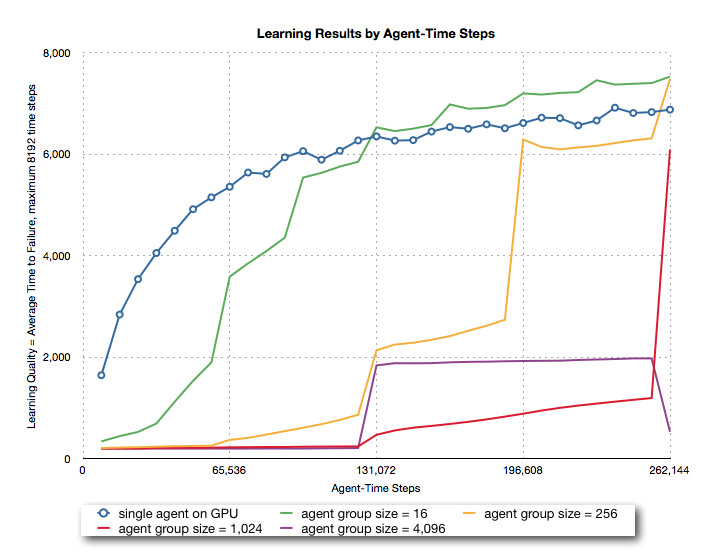
\includegraphics[scale=0.5]{fig07a}
\caption{Learning quality for Pole Balancing as a function of agent-time steps without agent differentiation.}
\label{fig:pole_steps}
\end{figure}

\begin{flushleft}

The frequency of sharing is a learning parameter that is determined separately by agent group size through experimentation.  As agent group size increases, the optimal number of time steps per agent between sharing decreases. 

The next measurements tested learning quality as a function of learning time.  As with the previous problem, learning time is measured based on a single run with the single agent on the CPU or group of parallel agents on the GPU.  The time spent testing the agent is, of course, excluded from the measurement.  The learning quality is then calculated by averaging the learning measurements over 1,024 trials.  The quality of learning with parallel agents is dramatically better than single agent learning for groups of 256 or larger when measured over a learning period of 200ms, as can be seen in Figure~\ref{fig:pole_time}


\end{flushleft}

\begin{figure}[hbtp]
\center
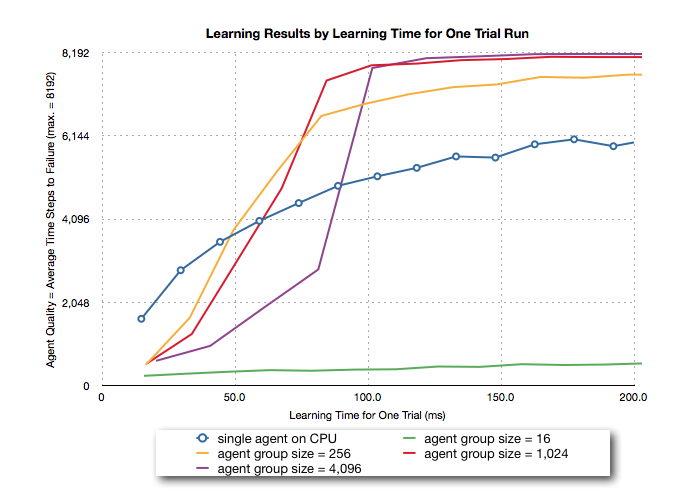
\includegraphics[scale=0.5]{fig08a}
\caption{Learning quality as a function of learning time for Pole Balancing, without agent differentiation.}
\label{fig:pole_time}
\end{figure}

\begin{flushleft}

Agent differentiation is beneficial to parallel learning for the Pole Balancing problem, as mentioned before.  The differentiation for each agent is a small random bias added to the $Q$-values shared with each agent. The amount of random bias was determined by experimentation and decreased exponentially over time.  Differentiation dramatically improves the speed of learning for agent groups of 256 or larger.  Figure~\ref{fig:pole_diff} shows the improvement that occurred during the first 100 ms of learning.  Ultimate quality does not change much because average quality is close to the best possible value of 8,192 and there is no room for improvement.  The final learning quality including the impact of differentiation is shown in Figure~\ref{fig:pole_timediff}, clearly showing the success of the parallel approach.

\end{flushleft}

\begin{figure}[hbtp]
\center
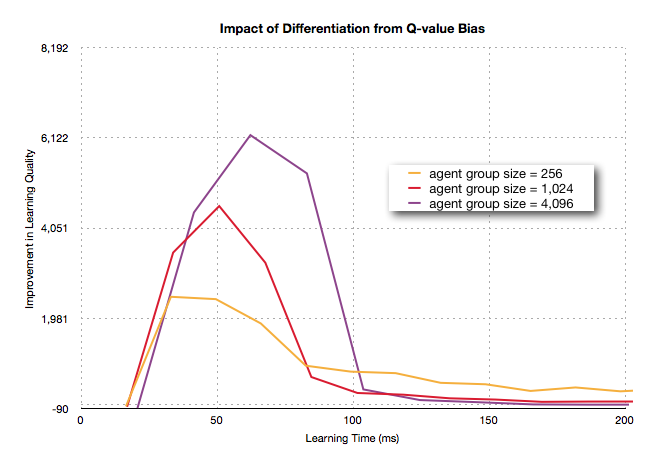
\includegraphics[scale=0.5]{fig09a}
\caption{}
\label{fig:pole_diff}
\end{figure}

\begin{flushleft}

\end{flushleft}

\begin{figure}[hbtp]
\center
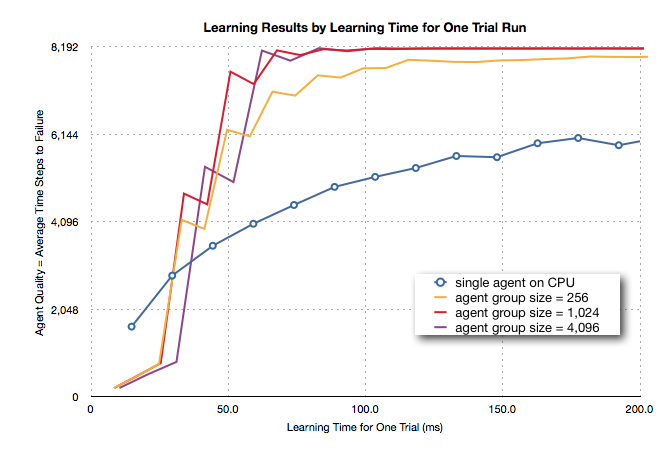
\includegraphics[scale=0.5]{fig10a}
\caption{}
\label{fig:pole_timediff}
\end{figure}

\begin{flushleft}

In summary, the massively parallel approach produces a dramatic improvement in learning quality as a function of the learning time for the Pole Balancing problem (Figure~\ref{fig:pole_timediff}).  This improvement is obtained by using information sharing and agent differentiation with groups of at least 256 parallel agents. 
